% Created 2022-07-14 Thu 16:54
% Intended LaTeX compiler: pdflatex
\documentclass[presentation,aspectratio=169]{beamer}
\usepackage[utf8]{inputenc}
\usepackage[T1]{fontenc}
\usepackage{graphicx}
\usepackage{grffile}
\usepackage{longtable}
\usepackage{wrapfig}
\usepackage{rotating}
\usepackage[normalem]{ulem}
\usepackage{amsmath}
\usepackage{textcomp}
\usepackage{amssymb}
\usepackage{capt-of}
\usepackage{hyperref}
\usepackage{khpreamble}
\usepackage{amssymb}
\usepackage{pgfplotstable}
\usepackage{pgfplots}
\pgfplotsset{compat=1.16}
\DeclareMathOperator{\shift}{q}
\DeclareMathOperator{\diff}{p}
\usetheme{default}
\author{Kjartan Halvorsen}
\date{\today}
\title{System identification}
\hypersetup{
 pdfauthor={Kjartan Halvorsen},
 pdftitle={System identification},
 pdfkeywords={},
 pdfsubject={},
 pdfcreator={Emacs 26.3 (Org mode 9.4.6)}, 
 pdflang={English}}
\begin{document}

\maketitle

\section{Intro}
\label{sec:org9403ba8}
\begin{frame}[label={sec:org1e78cfe}]{A complicated process}
\begin{columns}
\begin{column}{0.4\columnwidth}
\begin{center}
\includegraphics[height=0.7\textheight]{../../figures/Vertical-cyclone.jpg}
\end{center}

\footnotesize
From Wikipedia "Cyclonic separation"
\end{column}

\begin{column}{0.6\columnwidth}
\pause

 \begin{center}
 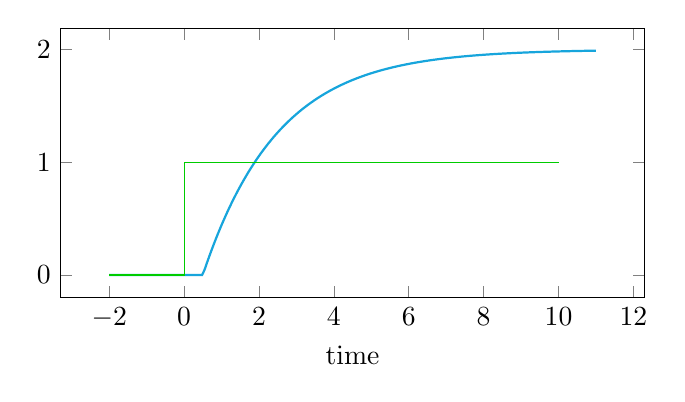
\begin{tikzpicture}

 \begin{axis}[%
 width = 9cm,
 height = 5cm,
 xlabel = time,
 ]
 \addplot+[thick,cyan!90!black, no marks, domain = -2:11, samples=200] {2*(x>0.5)*(1-exp(-(x-0.5)/2))};
 \addplot+[green!80!black, no marks] coordinates {(-2, 0) (0,0) (0,1) (10,1)};
\end{axis}
 \end{tikzpicture}
 \end{center}

Fit model \[G(s) = \frac{k\mathrm{e}^{-s\theta}}{\tau s + 1} \]
\end{column}
\end{columns}
\end{frame}

\begin{frame}[label={sec:org50f4fd8}]{System identification}
\begin{center}
  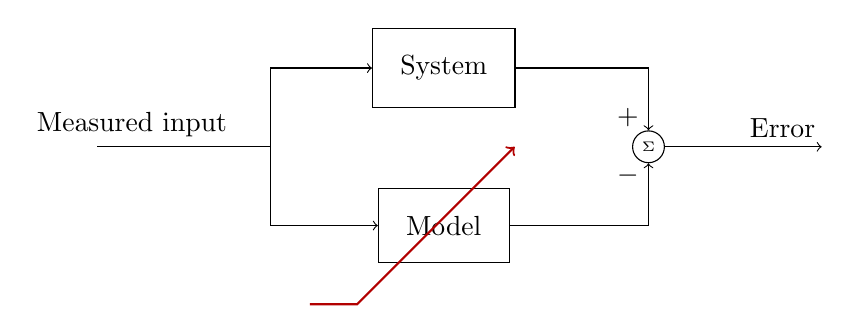
\begin{tikzpicture}[node distance=22mm, block/.style={rectangle, draw, minimum width=15mm, inner sep=10pt}, sumnode/.style={circle, draw, inner sep=2pt},]

    \node[coordinate] (input) {};
    \node[coordinate, right of=input] (copy) {};
    \node[coordinate, right of=copy] (midp) {};
    \node[block, above of=midp, node distance=10mm] (sys)  {System};
    \node[block, below of=midp, node distance=10mm] (mod)  {Model};
    \node[sumnode, right of=midp, node distance=26mm] (sum) {\tiny $\Sigma$};
    \node[coordinate, right of=sum, node distance=22mm] (output) {};

    \draw[-] (input) -- node[above, pos=0.2] {Measured input} (copy);
    \draw[->] (copy) |- node[above] {} (sys);
    \draw[->] (copy) |- node[above] {} (mod);
    \draw[->] (sys) -| node[left, pos=0.9] {$+$} (sum);
    \draw[->] (mod) -| node[left, pos=0.9] {$-$} (sum);
    \draw[->] (sum) -- node[above, near end] {Error} (output);

    \draw[thick, red!70!black, ->] (2.7,-2) -- (3.3,-2) -- (5.3, 0);
  \end{tikzpicture}
\end{center}
\end{frame}

\begin{frame}[label={sec:org6d47710}]{The Auto-Regressive with eXogenous input (ARX) model}
\begin{center}
\includegraphics[width=0.6\linewidth]{../../figures/block-arx}
\end{center}

\pause

\[ A(\shift) y(k) = B(\shift)u(k) + e(k+n) \]

The error signal \(e(k)\) is a zero-mean white noise sequence representing perturbations and modeling errors.
\end{frame}

\begin{frame}[label={sec:org4211b02}]{White noise}
\begin{center}
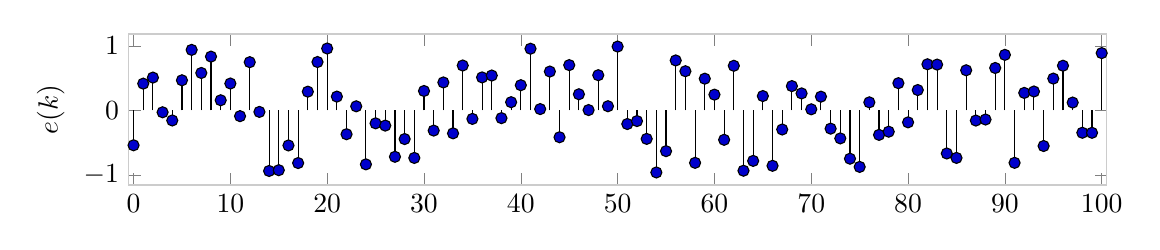
\begin{tikzpicture}
  \begin{axis}[axis line style={black!20},
  width=14cm,
  height=3.5cm,
  %xlabel={$t$},
  ylabel={$e(k)$},
  %xtick = {-1, 0, 1},
  %xticklabels={$k-1$, $k$, $k+1$},
  %xtick = {0, 2, 4, 6, 8, 10},
  %ytick=\empty,
  xmin=-.5,
  xmax=100.5,
]
  %\addplot[black, ycomb] table[x expr=\coordindex, y index=0] {\randntable};
  \addplot+[black, ycomb, domain=0:100, samples=101,variable=k] { rand}; 
\end{axis}
\end{tikzpicture}
\end{center}
\end{frame}

\begin{frame}[label={sec:org8d5caca}]{Random binary signal}
\begin{center}
\begin{tikzpicture}
  \begin{axis}[axis line style={black!20},
  width=14cm,
  height=3.5cm,
  %xlabel={$t$},
  ylabel={$u(k)$},
  %xtick = {-1, 0, 1},
  %xticklabels={$k-1$, $k$, $k+1$},
  %xtick = {0, 2, 4, 6, 8, 10},
  %ytick=\empty,
  %xmin=-.5,
  %xmax=100.5,
]
\addplot+[black, ycomb] table[x expr=\coordindex, y index=0] {../../figures/rbs_100.dta};

\end{axis}
\end{tikzpicture}
\end{center}
\end{frame}

\begin{frame}[label={sec:org43617b2}]{First-order ARX model with one delay}
\begin{center}
\includegraphics[width=0.3\linewidth]{../../figures/block-arx}
\end{center}
\[ (\shift + \textcolor{red!60!black!}{a_1}) y(k) = (\textcolor{red!60!black!}{b_0} \shift + \textcolor{red!60!black!}{b_1}) \shift^{-1}u(k) + e(k+1) \]
\[ y(k+1) +  \textcolor{red!60!black!}{a_1}y(k) = \textcolor{red!60!black!}{b_0}u(k) + \textcolor{red!60!black!}{b_1}u(k-1) + e(k+1) \]

\pause

Using the model to predict the output one step ahead:
\begin{align*}
 \hat{y}(k+1) &= -\textcolor{red!60!black!}{a_1}y(k) + \textcolor{red!60!black!}{b_0}u(k) + \textcolor{red!60!black!}{b_1}u(k-1) =  \underbrace{\begin{bmatrix} \textcolor{white}{-y(k)} & \textcolor{white}{u(k)} & \textcolor{white}{u(k-1)} \end{bmatrix}}_{\varphi_{k+1}^T} \underbrace{\begin{bmatrix} \textcolor{red!60!black}{a_1}\\\textcolor{red!60!black}{b_0}\\\textcolor{red!60!black}{b_1}\end{bmatrix}}_{\theta}\\
 &= \varphi_{k+1}^T\textcolor{red!60!black}{\theta}
 \end{align*}
\end{frame}





\begin{frame}[label={sec:org5aaa0d0}]{First-order ARX model with one delay}
\begin{center}
\includegraphics[width=0.3\linewidth]{../../figures/block-arx}
\end{center}
\[ (\shift + \textcolor{red!60!black!}{a_1}) y(k) = (\textcolor{red!60!black!}{b_0} \shift + \textcolor{red!60!black!}{b_1}) \shift^{-1}u(k) + e(k+1) \]
\[ y(k+1) +  \textcolor{red!60!black!}{a_1}y(k) = \textcolor{red!60!black!}{b_0}u(k) + \textcolor{red!60!black!}{b_1}u(k-1) + e(k+1) \]


Using the model to predict the output one step ahead:
\begin{align*}
 \hat{y}(k+1) &= -\textcolor{red!60!black!}{a_1}y(k) + \textcolor{red!60!black!}{b_0}u(k) + \textcolor{red!60!black!}{b_1}u(k-1) =  \underbrace{\begin{bmatrix} \textcolor{black}{-y(k)} & \textcolor{black}{u(k)} & \textcolor{black}{u(k-1)} \end{bmatrix}}_{\varphi_{k+1}^T} \underbrace{\begin{bmatrix} \textcolor{red!60!black}{a_1}\\\textcolor{red!60!black}{b_0}\\\textcolor{red!60!black}{b_1}\end{bmatrix}}_{\theta}\\
 &= \varphi_{k+1}^T\textcolor{red!60!black}{\theta}
 \end{align*}
\end{frame}




\begin{frame}[label={sec:orgc7266e2}]{Parameter estimation - Least squares}
\alert{Objective} Given observations \[\mathcal{D} = \{ (u_1,y_1), (u_2, y_2), \ldots, (u_N, y_N)\}\] and model \(\mathcal{M}: \; y(k+1) = -\textcolor{red!60!black!}{a}y(k) + \textcolor{red!60!black!}{b_0}u(k) + \textcolor{red!60!black!}{b_1}u(k-1)  + e(k+1)\), obtain the parameters \((\textcolor{red!60!black!}{a},\,\textcolor{red!60!black!}{b_0},\,\textcolor{red!60!black!}{b_1})\) which gives the best fit of the model to the data.
\end{frame}



\begin{frame}[label={sec:org91fe707}]{Parameter estimation - Least squares}
Given observations \[\mathcal{D} = \{ (u_1,y_1), (u_2, y_2), \ldots, (u_N, y_N)\}\] and model \(\mathcal{M}: \; y(k+1) = -\textcolor{red!60!black!}{a}y(k) + \textcolor{red!60!black!}{b_0}u(k) + \textcolor{red!60!black!}{b_1}u(k-1)  + e(k+1)\).

\begin{enumerate}
\item Form the one-step ahead prediction
\[ \hat{y}_{k+1} = -\textcolor{red!60!black!}{a_1}y_k + \textcolor{red!60!black!}{b_0}u_k + \textcolor{red!60!black!}{b_1}u_{k-1} =  \underbrace{\begin{bmatrix} -y_k & u_k & u_{k-1} \end{bmatrix}}_{\varphi_{k+1}^T} \underbrace{\begin{bmatrix} \textcolor{red!60!black!}{a_1}\\\textcolor{red!60!black!}{b_0}\\\textcolor{red!60!black!}{b_1}\end{bmatrix}}_{\textcolor{red!60!black!}{\theta}}\] and the prediction error
   \[ \epsilon_{k+1} = y_{k+1} - \hat{y}_{k+1} = y_{k+1} - \varphi_{k+1}^T\textcolor{red!60!black!}{\theta}.\]
\end{enumerate}
\end{frame}


\begin{frame}[label={sec:org0f4f9bf}]{Parameter estimation - Least squares}
\begin{enumerate}
\setcounter{enumi}{1}
\item Combine all the observations \(y_k\) and predictions \(\hat{y}_k\) on vector form
\begin{align*}
\epsilon &= \begin{bmatrix} \epsilon_3\\\epsilon_4\\\vdots\\\epsilon_N\end{bmatrix} =  \begin{bmatrix} y_3\\ y_4\\\vdots\\y_N \end{bmatrix} - \begin{bmatrix} \hat{y}_3\\ \hat{y}_4\\\vdots\\\hat{y}_N \end{bmatrix}
 =  \begin{bmatrix} y_3\\ y_4\\\vdots\\y_N \end{bmatrix} - \begin{bmatrix} \varphi_3^T\textcolor{red!60!black!}{\theta}\\ \varphi_4^T\textcolor{red!60!black!}{\theta}\\\vdots\\\varphi_N^T\textcolor{red!60!black!}{\theta} \end{bmatrix}\\
&= y - \underbrace{\begin{bmatrix}\varphi_3^T\\\varphi_4^T\\\vdots\\\varphi_N^T\end{bmatrix}}_{\Phi}\textcolor{red!60!black!}{\theta} = y - \Phi\textcolor{red!60!black!}{\theta} 
\end{align*}
\item Solve \(\arg\min \; J(\textcolor{red!60!black!}{\theta}) = \frac{1}{2}\epsilon^T\epsilon = \frac{1}{2}\sum_{i=3}^N \epsilon_i(\textcolor{red!60!black!}{\theta})^2\)
\end{enumerate}
\end{frame}


\begin{frame}[label={sec:org937f671}]{The problem with least squares}
\begin{columns}
\begin{column}{0.4\columnwidth}
\begin{center}
  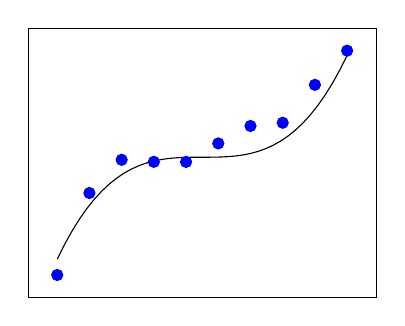
\begin{tikzpicture}
    \begin{axis}[
      width=6cm,
      height=5cm,
      %ylabel=loss,
      %xlabel=penalty,
      xtick = \empty,
      ytick = \empty,
      ]
      \addplot[black, no marks , domain=-2:2, samples=40] {x^3};
      \addplot[blue, only marks, domain=-2:2, samples=10] {x^3 + 2.3*rand};
    \end{axis}
  \end{tikzpicture}
\end{center}


\begin{align*}
 \text{minimize} \; &\sum_k g(\epsilon_k)\\
 \text{where} \; g(u) &= u^2
\end{align*}
\end{column}

\begin{column}{0.6\columnwidth}
\begin{center}
  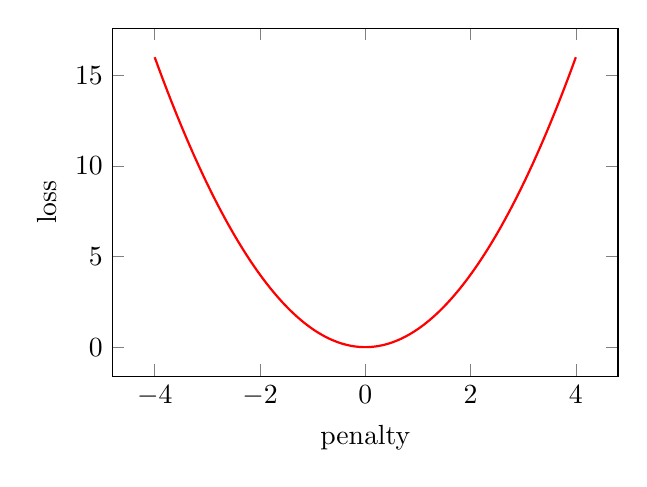
\begin{tikzpicture}
    \begin{axis}[
      width=8cm,
      height=6cm,
      ylabel=loss,
      xlabel=penalty,
      ]
      \addplot[red, thick, no marks, domain=-4:4, samples=201] {x^2};
    \end{axis}
  \end{tikzpicture}
\end{center}
\end{column}
\end{columns}
\end{frame}

\begin{frame}[label={sec:org86ffe3a}]{More robust: The Huber loss function}
\begin{columns}
\begin{column}{0.4\columnwidth}
Also known as \alert{robust regression}
\begin{align*}
 \text{minimize} \; &\sum_k g_{hub}(\epsilon_k)\\
 \text{where}\; g_{hub}(u) &= \begin{cases} u^2 & |u| \le M\\ M(2|u|-M) & |u| > M \end{cases}
\end{align*}
\end{column}

\begin{column}{0.6\columnwidth}
\begin{center}
  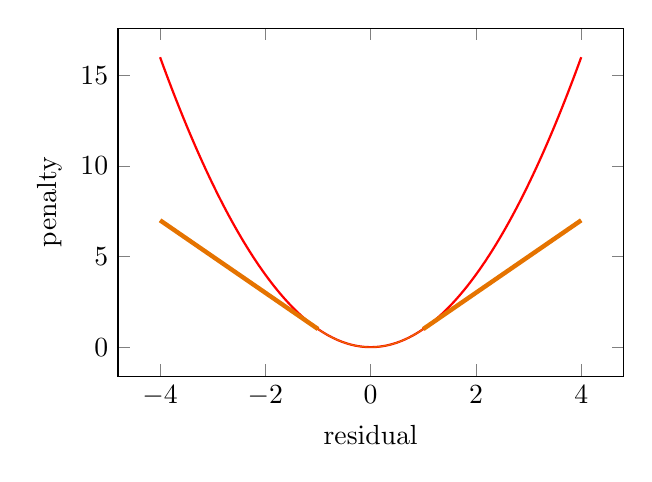
\begin{tikzpicture}
    \begin{axis}[
      width=8cm,
      height=6cm,
      ylabel=penalty,
      xlabel=residual,
      ]
      \addplot[red, thick, no marks, domain=-4:4, samples=201] {x^2};
      \addplot[orange!90!black, ultra thick, no marks, domain=-4:-1, samples=201] {2*abs(x)-1};
      \addplot[orange!90!black, thin, no marks, domain=-1:1, samples=201] {x^2};
      \addplot[orange!90!black, ultra thick, no marks, domain=1:4, samples=201] {2*abs(x)-1};
    \end{axis}
  \end{tikzpicture}
\end{center}
\end{column}
\end{columns}
\end{frame}


\begin{frame}[label={sec:orgf1667be}]{First-order ARX model without delay}
\begin{center}
\includegraphics[width=0.4\linewidth]{../../figures/block-arx}
\end{center}
\[ (\shift + \textcolor{red!60!black!}{a_1}) y(k) = (\textcolor{red!60!black!}{b_0} \shift + \textcolor{red!60!black!}{b_1}) u(k) + e(k+1) \]

\alert{Activity}

\begin{enumerate}
\item Determine the one-step ahead predictor \(\hat{y}_{k+1}\) and the prediction error \(\epsilon_{k+1}\).
\item Form the system of equations \(\Phi\textcolor{red!60!black!}{\theta} = y\)
\end{enumerate}
\end{frame}


\begin{frame}[label={sec:org3005953}]{The ARMAX model}
\[ A(\shift) y(k) = B(\shift)u(k) + C(\shift)e(k)\]

\alert{Activity} Fill the empty blocks.

\begin{center}
  \begin{tikzpicture}[node distance=22mm, block/.style={rectangle, draw, minimum width=15mm, minimum height=12mm}, sumnode/.style={circle, draw, inner sep=2pt}]
    
    \node[coordinate] (input) {};
    \node[block, right of=input, node distance=20mm] (plant)  {};
    \node[sumnode, right of=plant, node distance=24mm] (sum) {\tiny $\Sigma$};
    \node[block, above of=sum, node distance=20mm] (dist)  {};

    \node[coordinate, above of=dist, node distance=12mm] (disturbance) {};
    \node[coordinate, right of=sum, node distance=20mm] (output) {};

    \draw[->] (input) -- node[above, pos=0.3] {$u(k)$} (plant);
    \draw[->] (plant) -- node[above] {} (sum);
    \draw[->] (sum) -- node[above, near end] {$y(k)$} (output);
    \draw[->] (disturbance) -- node[right, pos=0.2] {$e(k)$} (dist);
    \draw[->] (dist) -- node[above] {} (sum);

  \end{tikzpicture}
\end{center}
\end{frame}
\end{document}